\documentclass[14pt]{extreport}  
\usepackage{fontspec}  
\usepackage{polyglossia}  
\setmainlanguage{russian}  
\setotherlanguages{english}  
\setmainfont{Times New Roman}  
\usepackage[a4paper,left=30mm,right=10mm,top=20mm,bottom=20mm]{geometry}
\setlength{\parindent}{1.25cm}
\usepackage{indentfirst}
\setlength{\parindent}{1.25cm}
\setlength{\parskip}{0pt}
\linespread{1.5}
\usepackage{fancyhdr}
\pagestyle{fancy}
\fancyhf{}
\fancyfoot[C]{\thepage}
\usepackage{graphicx}
\usepackage{hyperref}  
\begin{document}
\title{Реферат на тему: \\[0.5cm] \textbf{Итераторы в Python}}
\author{Студентка: Васильева Елизавета Дмитриевна \\ Группа: 2.1}
\date{17.09.2024}
\thispagestyle{empty}
\maketitle
\chapter{Введение}  
\sloppy

Итераторы — это ключевой концепт в Python, который позволяет создавать и работать с последовательностями объектов. Они являются основой многих встроенных структур данных, таких как списки, кортежи и множества, а также используются для создания пользовательских структур данных.

\chapter{Основная часть - 1}  
\section{Раздел 1.1}  
\sloppy
\textbf{Итератор} — это объект, который реализует два метода: iter и next. Метод iter возвращает сам итератор, а метод next возвращает следующий элемент в последовательности. Если в последовательности больше нет элементов, метод next должен вызвать исключение StopIteration. Пример итератора изображен на картинке \ref{fig:image1}.

\begin{figure}[ht]
\centering
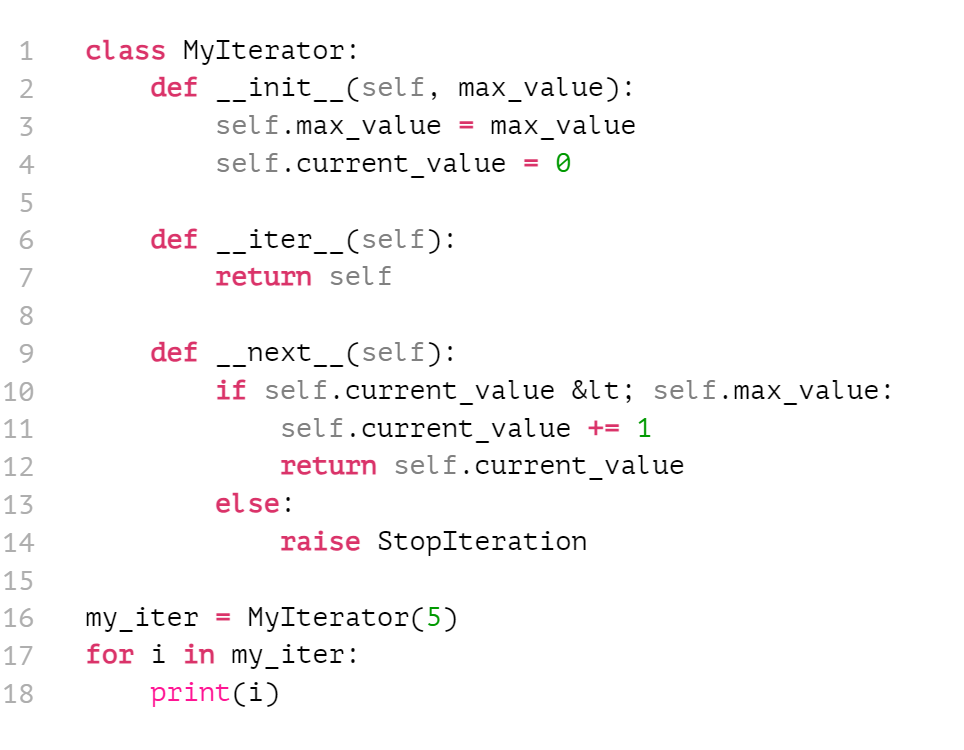
\includegraphics[width=0.5\textwidth]{image1.png}
\caption{Пример простого итератора}
\label{fig:image1}
\end{figure}




\subsection{Подраздел 1.1.1}  
\sloppy
В Python итераторы используются с помощью ключевого слова \textit{for}. Оно позволяет перебирать элементы последовательности, вызывая метод next для каждого элемента до вызова исключения \underline{StopIteration}. Итераторы в Python можно использовать не только для встроенных структур данных, но и для пользовательских. Это позволяет создавать более сложные и гибкие структуры данных, которые могут быть обработаны с помощью стандартного синтаксиса \textit{for}.

\subsection{Подраздел 1.1.2}  
\sloppy

Стоит отдельно остановиться на том, что цикл \textit{for}, в Python, устроен несколько иначе, чем в большинстве других языков. Он больше похож на \textit{for...each}, или же \textit{for...of}.
Если же, мы перепишем цикл for с помощью цикла while, используя индексы, то работать такой подход будет только с последовательностями. А с итерируемыми объектами, последовательностями не являющимися, не будет.

\subsection{Подраздел 1.1.3}  
\sloppy

Теперь формализуем протокол итератора целиком:

\begin{enumerate}
\item Чтобы получить итератор мы должны передать функции iter итерируемый объект.
\item Далее мы передаём итератор функции next.
\item Когда элементы в итераторе закончились, порождается исключение StopIteration.
\end{enumerate} 

Особенности:
\begin{enumerate}
\item Любой объект, передаваемый функции iter без исключения TypeError — итерируемый объект.
\item Любой объект, передаваемый функции next без исключения TypeError — итератор.
\item Любой объект, передаваемый функции iter и возвращающий сам себя — итератор.
\end{enumerate}

Плюсы итераторов:
Итераторы работают "лениво" . А это значит, что они не выполняют какой-либо работы, до тех пор, пока мы их об этом не попросим. Таким образом, мы можем оптимизировать потребление ресурсов ОЗУ и CPU, а так же создавать бесконечные последовательности.

\section{Раздел 2}  
\sloppy
Для сравнения удобства различных моделей итераторов на практике были реализованы итераторы для нескольких типовых задач и результаты этого сравнения свели в следующую таблицу \ref{tab:example}
(«+» означает «удобно», «−» — неудобно и «0» — не очень удобно.)
\begin{table}[h]
\centering
\begin{tabular}{|c|c|c|c|}
\hline
Язык & Массив/Диапозон & Связный список  & Чтение файла по строкам   \\
\hline
С & + & 0  & 0   \\
\hline
Python & + & 0  & +   \\
\hline
Java & + & 0  & -   \\
\hline
yield & + & +  & +   \\
\hline
\end{tabular}
\caption{Сравнительная таблица}
\label{tab:example}
\end{table} 

\chapter{Заключение}  
\sloppy
Итераторы — это мощный инструмент в Python, который позволяет работать с последовательностями объектов. Они используются для перебора элементов встроенных структур данных, таких как списки и кортежи, а также для создания пользовательских структур данных. Используйте итераторы для упрощения работы с последовательностями объектов и для повышения гибкости вашего кода.
\begin{figure}[h]
\centering
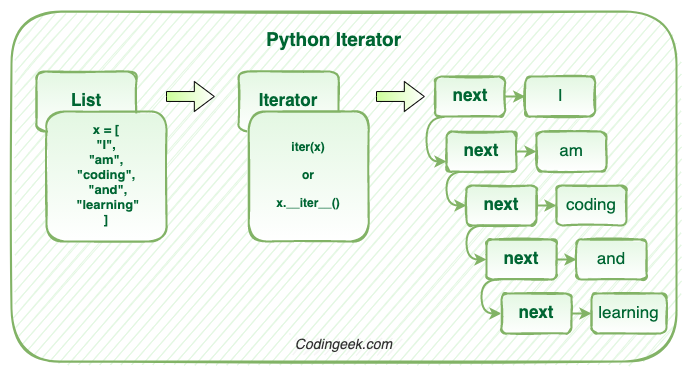
\includegraphics[width=0.5\textwidth]{example-image.png}
\label{fig:example}
\end{figure}

\tableofcontents
\section{Список литературы}
\begin{enumerate}
\item \href{https://habr.com/ru/articles/840068/}{ Статья на Habr} 
\item \href{https://sky.pro/media/chto-takoe-iteratory-i-kak-ih-ispolzovat-v-python/}{ Статья Алексея Кодова} 
\end{enumerate}

\end{document}
